%%%%%%%%%%%%%%%%%%%%%%%%%%%%%%%%%%%%%%%%%
% baposter Landscape Poster
% LaTeX Template
% Version 1.0 (11/06/13)
%
% baposter Class Created by:
% Brian Amberg (baposter@brian-amberg.de)
%
% This template has been downloaded from:
% http://www.LaTeXTemplates.com
%
% License:
% CC BY-NC-SA 3.0 (http://creativecommons.org/licenses/by-nc-sa/3.0/)
%
%%%%%%%%%%%%%%%%%%%%%%%%%%%%%%%%%%%%%%%%%
% !TEX TS-program = pdflatex
%----------------------------------------------------------------------------------------
%	PACKAGES AND OTHER DOCUMENT CONFIGURATIONS
%----------------------------------------------------------------------------------------

\documentclass[landscape,a0paper,fontscale=0.285]{baposter} % Adjust the font scale/size here

\usepackage{graphicx} % Required for including images
\graphicspath{{figures/}} % Directory in which figures are stored

\usepackage{mathrsfs}  
\usepackage{amsmath} % For typesetting math
\usepackage{amssymb} % Adds new symbols to be used in math mode

\usepackage{booktabs} % Top and bottom rules for tables
\usepackage{enumitem} % Used to reduce itemize/enumerate spacing
\usepackage{palatino} % Use the Palatino font
\usepackage[font=small,labelfont=bf]{caption} % Required for specifying captions to tables and figures

\usepackage{multicol} % Required for multiple columns
\setlength{\columnsep}{1.5em} % Slightly increase the space between columns
\setlength{\columnseprule}{0mm} % No horizontal rule between columns

\usepackage{tikz} % Required for flow chart
\usetikzlibrary{shapes,arrows} % Tikz libraries required for the flow chart in the template

\newcommand{\compresslist}{ % Define a command to reduce spacing within itemize/enumerate environments, this is used right after \begin{itemize} or \begin{enumerate}
\setlength{\itemsep}{1pt}
\setlength{\parskip}{0pt}
\setlength{\parsep}{0pt}
}

\definecolor{uofsgreen}{rgb}{.125 .5 .25} % Defines the color used for content box headers

\begin{document}

\begin{poster}
{
headerborder=closed, % Adds a border around the header of content boxes
colspacing=1em, % Column spacing
bgColorOne=white, % Background color for the gradient on the left side of the poster
bgColorTwo=white, % Background color for the gradient on the right side of the poster
borderColor=uofsgreen, % Border color
headerColorOne=black, % Background color for the header in the content boxes (left side)
headerColorTwo=uofsgreen, % Background color for the header in the content boxes (right side)
headerFontColor=white, % Text color for the header text in the content boxes
boxColorOne=white, % Background color of the content boxes
textborder=roundedleft, % Format of the border around content boxes, can be: none, bars, coils, triangles, rectangle, rounded, roundedsmall, roundedright or faded
eyecatcher=true, % Set to false for ignoring the left logo in the title and move the title left
headerheight=0.1\textheight, % Height of the header
headershape=roundedright, % Specify the rounded corner in the content box headers, can be: rectangle, small-rounded, roundedright, roundedleft or rounded
headerfont=\Large\bf\textsc, % Large, bold and sans serif font in the headers of content boxes
%textfont={\setlength{\parindent}{1.5em}}, % Uncomment for paragraph indentation
linewidth=2pt % Width of the border lines around content boxes
}
%----------------------------------------------------------------------------------------
%	TITLE SECTION 
%----------------------------------------------------------------------------------------
%
{
\includegraphics[height=4em]{UofS}} % First university/lab logo on the left
{\bf\textsc{Designing error control circuits for 4-qubit quantum computer}\vspace{0.5em}} % Poster title
{\hspace{85pt}\textsc{Marina Schmidt \hspace{50pt}  Department of Computer      \\and Raymond Spiteri\hspace{110pt}       Science}} % Author names and institution
{
\includegraphics[height=4em]{NRSL-Mesh2-01.png}} % Second university/lab logo on the right

%----------------------------------------------------------------------------------------
%	INTRODUCTION
%----------------------------------------------------------------------------------------


\headerbox{Introduction}{name=introduction,column=0,span=1,row=0}{
  \documentclass{article}
\usepackage[utf8]{inputenc}
\usepackage{authblk}
\usepackage{amsmath}

\title{Designing error control circuits for 4-qubit quantum computing}
\author[1]{Marina Schmidt}
\author[1]{Dr. R. Spiteri}
\affil[1]{Department of Computer Science, University of Saskatchewan}
\affil[ ]{Email: \textit {mts299@mail.usask.ca}}
\affil[ ]{NSID: mts299}

\begin{document}

\maketitle

\section{Introduction}
 Quantum computers hold a promising advantage to solving hard problems, such as prime factorization, within a sufficient amount of time. This is because of their ability to harness the quantum states of subatomic particles (e.g. photons and electrons) to represent a quantum bit (qubit). Similar to a classical bit, a qubit can represent zero or one state based on their subatomic properties (e.g, spin); however, a qubit can also be in both states when not being measured because of quantum superposition. Because of this quantum property, when a qubit is added to the system it can interact with the other qubits to create superposition states that will increase the amount of information provided to the system. For example, a two qubit system can be represented as: 
\begin{align*}
&\delta |11\big\rangle \\ 
&\gamma |01 + 10 \big\rangle \\
&\beta  |01 - 10 \big\rangle \\
&\alpha |00 \big\rangle \\
&\end{align*}
Therefore, four bits of information ($\alpha,\beta,\gamma$ and $\delta$) are required to describe the system, whereas a two bit classical system only takes two bits of information to describe the system. With this property of superposition, entanglement of qubits can allow an exponential of two to represent the information. However, when the system state is measured the qubit system has to fall into one of the basis states ($|11\big\rangle$ or $|00 \big\rangle$). To determine the superposition state the qubit system coherence pulse can be measured by using a series of logical operations. 

The ability of the qubit to interact with other qubit is also problematic because it can interact with other environmental subatomic particles from which it is impossible to isolate a qubit system. When this undesired interaction occurs, decoherence or loss of information causes errors in the information read from the system. Decoherence creates a dampening affect on the resulting pulse read from the qubit system when this dampening hits a flat line, decoherence time, all information is lost from the system. To prevent the major loss of information from decoherence, error correction operations are applied to obtain the resulting information from the system. One constraint on this is the error correction time needs to be less than decoherence time. Another constraint on error correction in a qubit system is it cannot use redundancy similar to classical bit error correction because of the no-cloning theorem. This theorem states that one cannot clone a qubit system because of uncertantity in the superposition states. Therefore another method of error correction needs to be designed to handle the quantum noise and decoherence of the system. 

To obtain fault tolerance in a qubit system, several models of circuit operations to be applied to the qubit system have been designed. These models use circuit constants that manipulate frequencies in the qubit system to obtain the corrected readings of the qubit system. The overall reading can then be used to obtain an intrinsic fidelity. The intrinsic fidelity is without circuit noise and it is used to theoretically determine the reliability of the circuit gate design. Therefore by optimizing the gate constants to obtain the desired fidelity, a designed circuit gate for error correction can be used to create a fault tolerant qubit system. 

In this poster the Tofolli single shot gate is optimized to obtain an intrinsic fidelity of $99.99\%$. It promises enough robustness in the error correction gate to guarantee fault tolerance without losing too much gate time so as to stay lower than the decoherence time. The four qubit system is examined in this poster because it lowest enough system to create encoding codes for encryption and logical operations in quantum machine that then can be taken advantage of in five qubit system for the overall decryption process for security applications. By optimizing the tofolli single shot security for a four qubit system with an intrinsic fidelity of $99.99\%$, this circuit design can be used for further research into quantum encryption.              
\end{document}


}


\headerbox{Figure 1}{name=figure1,column=2,span=1,row=0}
{
  \begin{center}
        \scalebox{0.35}{
            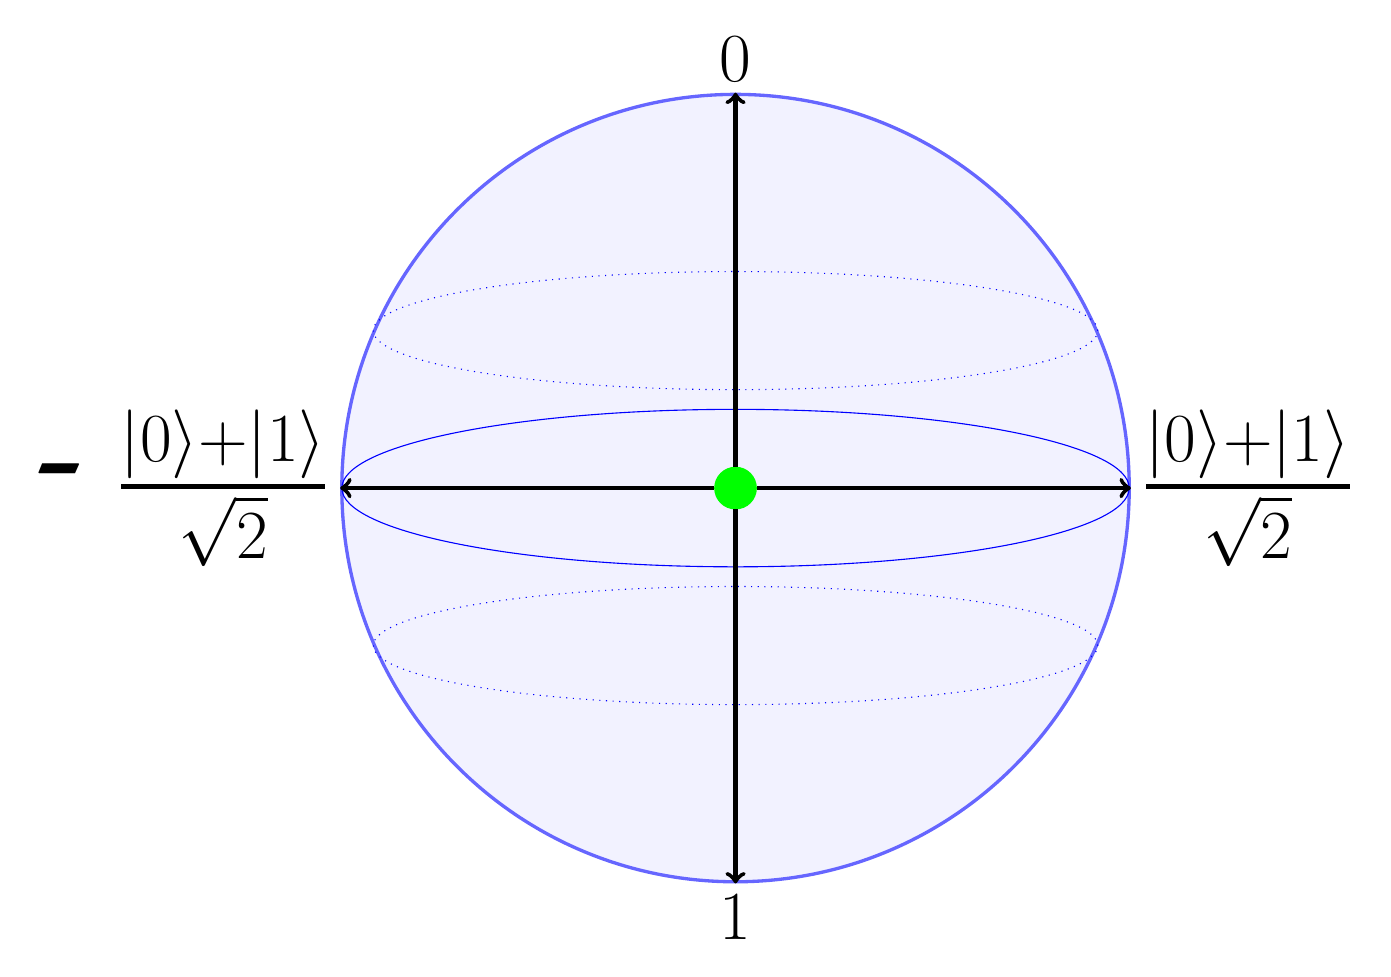
\begin{tikzpicture}[
                    roundnode/.style={circle, draw=green, fill=green, very thick, minimum size=0.5cm},
                    Largenode/.style={circle, draw=blue!60, fill=blue!5, very thick, minimum size=10cm},
                    ovalnode/.style={ellipse, fill=black,ultra thick, draw=black, minimum width=10cm,minimum length=5cm}
                    text/.style={text width=5cm}
                ]
                %Nodes
                \node[Largenode]        (largecircle)   {};
                \node[roundnode]        (main)                                                  {};
                \draw[blue] (0,0) ellipse (5 and 1);
                \draw[blue, dotted] (0,2) ellipse (4.6 and 0.75);
                \draw[blue, dotted] (0,-2) ellipse (4.6 and 0.75);
                \draw[->, ultra thick]  (main.north) -- (largecircle.north) node[above,font=\fontsize{50}{50}\selectfont] {$0$};
                \draw[->, ultra thick]  (main.east) -- (largecircle.east) node[right,font=\fontsize{50}{50}\selectfont]  { $\frac{|0\rangle+|1\rangle}{\sqrt{2}}$};
                \draw[->, ultra thick]  (main.west) -- (largecircle.west) node[left,font=\fontsize{50}{50}\selectfont] {- $\frac{|0\rangle+|1\rangle}{\sqrt{2}}$};
                \draw[->, ultra thick]  (main.south) -- (largecircle.south) node[below,font=\fontsize{50}{50}\selectfont] {$1$};



            \end{tikzpicture}
          }
        \end{center}
}

\headerbox{Toffolli single shot model}{name=details1,column=1,span=1,row=0}{
  The CCZ gate is component of the toffoli single shot circuit that deals with error correction. The gate can be repersented as a controlled Hamiltonian matrix as a vector operator: $\mathbf{\hat{H}^c}$, that is influenced by the controlled parameters $\varepsilon (t)$. These parameters determine the phase of the frequency to correct the qubit system with. The drift Hamiltonian, $\hat{H}^{dr}$ then reperesent the non-controlled qubit system. Therefore, the overall Hamiltonian of the qubit system
is reperesented as: 
\begin{equation*}
\hat{H} \big( \varepsilon (t) \big) = \hat{H}^{dr} + \varepsilon (t) \cdot  \mathbf{\hat{H}^c}
\end{equation*}

The system can further be expressed over time by unitary evolution operator:
\vspace{0.15cm}
\begin{align*}
  \tilde{U}(\varepsilon(t);\tau) = T e^{\Big( -i \int_{0}^{\tau} \hat{H}(\varepsilon(t))dt \Big) } 
\end{align*}
To determine how well the system is corrected, the target unitary evolution operator, $U$, is chosen based on the gate design. The fidelity of the simulation is then defined as:
\begin{center}
\begin{align*}
  \mathscr{F} (\varepsilon(t)) = \frac{1}{N} Re \Big(Tr \big(U\tilde{U}(\varepsilon(t))\big) \Big)
\end{align*}
\end{center}
Representing the objective function that optimizes for the maximum intrinsic fidelity that exceeds $99.99\%$. 




}



%----------------------------------------------------------------------------------------
%	DETAILS
%----------------------------------------------------------------------------------------
\headerbox{Optimization scheme}{name=details2,column=2,span=1,row=0,below=figure1}{
  \usepackage{mathrsfs}
\section{Method}

The chosen software to solve this problem was Global Search from MATLABs global optimization toolbox because of the ability to apply constraints. The constraint in four qubit system is that the intrinsic fidelity determined calculated by the model needs only to exceed $99.99\%$ to be consider satisfiable for experimentation.
\begin{equation}
  \mathsc{F}\big(\varepsilon(t)\big) \geq 0.9999
  \label{constraint}
\end{equation}
 This is because of the trade off between overall gate time for correcting the system and acceptable level of robustness for fault tolerance. As well
the constraint that the overall gate processing time cannot be exceed the decoherence time or else error correction can not be achieved. 

As shown in Figure \ref{globalsearch}, the global search algorithm is hybrid method that uses fmincon as the local solver. The objective function in this optimization scheme is defaulted to zero: 
\begin{equation}
  f(x) = 0
\end{equation}
where the actual calculation is done in the constraint (Eq.~\ref{constraint}) function. 

Previous attempts have been made to solve the four qubit system with a simple optimization scheme by solving for the maximum fidelity value:
\begin{equation}
  max \big(\mathsc{F}\big) 
\end{equation}




}

\headerbox{3-Qubit pulse signal}{name=figure2,column=2,span=1,row=0,below=details2,above=bottom}
{
  \begin{center}
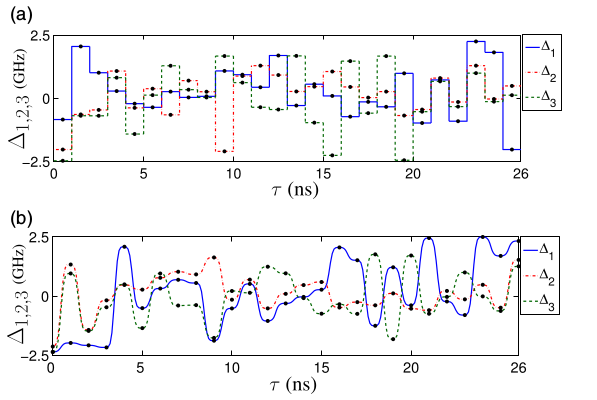
\includegraphics[width=7.25cm]{fidelity}
\end{center}
}


\headerbox{2-Qubit interaction}{name=figure3,column=1,span=1,row=0,below=details2,above=bottom}
{
  \vspace{0.37cm}
  \begin{center}
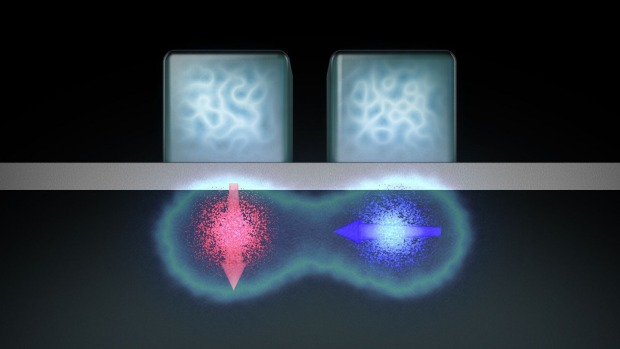
\includegraphics[width=7.25cm]{2qubit.jpg}
\end{center}
}

%----------------------------------------------------------------------------------------
%	RESULTS AND CONCLUSIONS
%----------------------------------------------------------------------------------------

\headerbox{Results \& Conclusions}{name=resultsandconclusions,column=3}{ % This block's bottom aligns with the bottom of the details block, add bottomaligned=details in need
	
  By approaching the problem as a feasibility problem, we have been success in obtaining processing times for the error correction gate up to $65$ nano seconds. The following Table~\ref{tab:4 qubit results} show currently running time gates and their current status of highest fidelity.  

\begin{table}[H]
    \caption{Four qubit intrinsic fidelity results}
    \centering
    \begin{tabular}{c|c|c}
    \hline  $T$ $(ns)$  & Intrinsic fidelity & CPU time \\
    \hline
    $150$ &$1.0$      &1 week\\
    $120$ &$0.999977$ &1 week \\
    $75$  &$0.999908$ &1 week\\
    $74$  & $0.9999546$ & 13 days\\
    $70$  & $0.9999795$ & 3 months \\
    $65$  & $0.9999785$ & 3 months \\ \hline

    \end{tabular}
    \label{tab:4 qubit results}
\end{table}

With success of this method of approaching this problem were proceeding to use a global optimization solver from pythOPT, a python problem solving environment, to solve this problem as well looking into to lower and higher qubit systems. 


\begin{table}[H]
    \caption{Four qubit intrinsic fidelity results}
    \centering
    \begin{tabular}{c|c|c}
    \hline  $T$ $(ns)$  & Intrinsic fidelity & CPU time \\
    \hline
    $27$  & $0.999992$ &1 day \\
    $26$  & $0.9999  $ &1 month\\
    $25$  & $0.994626$ &1 month\\
    $23$  & $0.974143$ & 1 month \\
    $20$  & $0.935444$ & 1 month\\
    $15$  & $0.907205$ & 1 month\\
    $10$  & $0.843589$ & 1 month \\ \hline


    \end{tabular}
    \label{tab:3 qubit results}
\end{table}

\begin{table}[H]
    \caption{Four qubit intrinsic fidelity results}
    \centering
    \begin{tabular}{c|c|c}
    \hline  $T$ $(ns)$  & Intrinsic fidelity & CPU time \\
    \hline
    $500$  &$0.305841$ &2 week\\
    $300$  &$0.41861$  &2 week \\
    $250$  &$0.295303$ &1 month\\
    $200$  &$0.608859$ &1 month\\
    $200$  &$0.868338$ &1 month\\ \hline


    \end{tabular}
    \label{tab: 5 qubit results}
\end{table}

By optimizing this problem as a feasibility problem we are able to obtain solutions for three and four qubit system, bring a new approach to optimizing quantum error corrections simulations. These give a promising design to a circuit that will be place on quantum processor chip. These chips can then be dedicated to encoding bit strings for security purposes that are using quantum networks. Likewise, furthers our understanding of optimizing for quantum error correction simulation and pushing
to solve the five-qubit system. Striving to solve the five-qubit system is the next step to design a stable decoding gate to match the four-qubit encoding gate. 


  \chapter{Conclusion}
\label{Conclusion}

I conclude that I have solved the problem! 

}

%----------------------------------------------------------------------------------------
%	REFERENCES
%----------------------------------------------------------------------------------------
%
%\headerbox{References}{name=references,column=0,span=3,row=1,align=contact,below=introduction}{
%
%\renewcommand{\section}[2]{\vskip 0.05em} % Get rid of the default "References" section title
%\nocite{*} % Insert publications even if they are not cited in the poster
%\small{ % Reduce the font size in this block
%\bibliographystyle{unsrt}
%\bibliography{sample} % Use sample.bib as the bibliography file
%}}
%
%----------------------------------------------------------------------------------------
%	FUTURE RESEARCH
%----------------------------------------------------------------------------------------


%----------------------------------------------------------------------------------------
%	CONTACT INFORMATION
%----------------------------------------------------------------------------------------



\headerbox{Future Research}{name=future,column=3,span=1,below=resultsandconclusions}{ % This block is as tall as the references block

  \section{Future work}

With this new scheme of optimizing the qubit system further work is being done on to minimize the gate time, as well a way to reformulate the objective function to consider the gate processing time; currently set as parameter before the optimization. 

Another system to solve is the five qubit system; by solving this system the four qubit system can be used for encoding purposes in quantum computers and the five qubit system will decode the message. This can lead into using quantum computers for security for the main computer calculations and even the internet purposes. 




}


\headerbox{Contact Information}{name=contact,column=0,below=introduction,above=bottom}{ % This block is as tall as the references block

\begin{description}\compresslist
\item[Web] simlab.usask.ca
\item[Email] mts299@mail.usask.ca
\item[Phone] +1 (306) 716-3561
\end{description}
}


%----------------------------------------------------------------------------------------

\end{poster}

\end{document}
